\documentclass[book]{deliverablereport}
\usepackage[style=alphabetic,backend=bibtex]{biblatex}
\addbibresource{../../lib/kbibs/kwarcpubs.bib}
\addbibresource{../../lib/kbibs/extpubs.bib}
\addbibresource{../../lib/kbibs/kwarccrossrefs.bib}
\addbibresource{../../lib/kbibs/extcrossrefs.bib}
\addbibresource{../../lib/deliverables.bib}
\addbibresource{local.bib}
%\usepackage{local}
\usepackage[show]{ed}
\usepackage{stex-logo}
\usepackage{rotating}

\title{Curated Math-in-the-Middle Ontology and Alignments for GAP/SAGE/LMFDB}
\def\shorttitle{Curated MitM Ontology/Alignments}

\deliverable{dksbases}{lfmverif}
\deliverydate{1/07/2018}
\duedate{1/09/2018}

\author{John Cremona}
\author{Dennis M\"uller}
\author{Michael Kohlhase}
\author{Markus Pfeiffer}
\author{Florian Rabe}
\author{Nicolas Thierry}
\author{Tom Wiesing}

\begin{document}
\begin{abstract}
  This Report describes the Math-in-the-Middle (MitM) Ontology developed in the
  OpenDreamKit project. It serves as a reference and pivotal point for translations
  between the various input languages of mathematical software systems. 
\end{abstract}
\maketitle
%\newpage\strut\githubissuedescription
\newpage\tableofcontents\newpage

\section{Introduction}
The Math-in-the-Middle (MitM) Ontology developed in the OpenDreamKit project. It serves as
a reference and pivotal point for translations between the various input languages of
mathematical software systems. This integration and interoperability has been described
in~\cite{DehKohKon:iop16,WieKohRab:vtuimkb17,KohMuePfe:kbimss17} and -- in great detail --
in \cite{ODK-D6.5}. In a nutshell, the MitM Ontology describes the mathematical objects,
concepts, and their relations in a general, system-agnostic way in an OMDoc/MMT theory
graph while the mathematical systems export API theories that describe the system
interface language in terms of types, classes, constructors, and functions -- again in
OMDoc/MMT. These two levels of descriptions are linked by OMDoc/MMT
alignments~\cite{MueGauKal:cacfms17} that allow the translation of expressions in the
interface language of system $A$ into the MitM-induced language, and from there to the
interface language of system $B$~\cite{MueRoYuRa:abtafs17}.

\section{The MitM Ontology and Interface Theories}
The Math-in-the-Middle Ontology is hosted on the MathHub.info system
\url{http://mathhub.info}, the sources can be obtained from
\url{http://gl.mathhub.info}. As the MathHub front-end is currently undergoing major
re-write\footnote{The old MathHub interface was based on Drupal, which led to major system
  vulnerabilities and therefore maintenance hassles, because Drupal was targeted by
  hackers. We are currently working on a docker-based orchestration of services with a
  React.JS based front-end in the general spirit of the OpenDreamKit VRE toolkit; see
  \url{https://github.com/MathHubInfo/}. The new system can be accessed at
  \url{http://new.mathhub.info}.} we will reference the MitM ontology by its sources --
the semantically enhanced user interface can be accessed via the same URLs without the
\url{gl.} part.\ednote{See how far we get, and maybe change the URLs}

The development consists of three parts:
\begin{compactenum}[\em i\rm)]
\item the MitM ontology which has the formalization of mathematical background theories,
\item the SMGloM Glossary which has informal, but semantically structured versions of the
  same content, and can therefore act as a human-readable documentation, and the
\item System API theories for the OpenDreamKit Systems and mathematical data bases. 
\end{compactenum}
We will discuss all three parts separately below.

\subsection{The MitM Ontology}

The MitM Ontology can be found at
\url{https://gl.mathhub.info/MitM/}, it comes in three parts:
\begin{itemize}
\item The \textbf{MitM foundation} in the archive \href
  {https://gl.mathhub.info/MitM/foundation}{\texttt{foundation}} (4 files, 539k LoF (lines
  of formalization), 103 commits). It contains the basic representational infrastructure
  used in the MitM ontology: a powerful higher-order logic with dependent record types,
  subtyping, and flexary function application (sequence arguments).
\item The \textbf{MitM core} in the
  \href{https://gl.mathhub.info/MitM/smglom}{\texttt{smglom}}\footnote{The name
    \texttt{smglom} was initially chosen for the ``Semantic Multilingual Glossary of
    Mathematics'' (SMGloM; see \ref{sec:smglom} below) with which it is
    cross-referenced. We will rethink naming once the MitM Ontology stabilizes.}  archive
  (43 files, 2600 LoF, 370 commits). This carries the bulk of knowledge representation in
  the MitM Ontology . The main thrust of curation has been to get the VRE use cases
  reported on in~\cite{ODK-D6.5}, but we also have elementary formalizations of algebra,
  arithmetics, calculus category theory, set collections, elliptic curves (for LMFDB),
  functional-analysis, geometry, graph theory, measure theory, set theory, and topology.
\item The \textbf{Modeling and Simulation Ontology} in the
  \href{https://gl.mathhub.info/MitM/smglom}{\texttt{models}} archive (11 files, 650 LoF,
  113 commits). This is an experimental extension of the MitM ontology, where we test the
  MitM framework (and the OpenDreamKit technologies) for modeling and simulation in
  opto-electronics.
\end{itemize}
There are various other archives in the \href{https://gl.mathhub.info/MitM/}{\texttt{MitM}
  library}, they are experiments, where the MitM ontology has been picked up by other
projects.

The MitM Ontology formalizations are very information-rich; see Figure~\ref{fig:mitm1} for
an example from computational group theory. 

\begin{figure}[ht]\centering
  \fbox{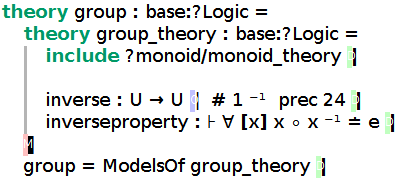
\includegraphics[width=8cm]{../MACIS17-interop/mitm1}}
  \caption{A Formalization of a Group}\label{fig:mitm1}
\end{figure}

\subsection{The ``Semantic Multilingual Glossary of Mathematics'' (SMGloM)}\label{sec:smglom}
The SMGloM library is available at \url{https://gl.mathhub.info/smglom}. It contains
ca. 815 glossary modules (OMDoc/MMT theories) with more than 1700 concepts. All
represented in \sTeX, a semantic variant of {\LaTeX} developed by FAU and
JacU. Figure~\ref{fig:conductor} shows an example. The boldface words are definienda
(i.e. concepts to be defined; here ``conductor'') and the blue ones are concepts already
defined in other parts of the MitM Ontology. SMGloM definitions are multilingual -- mostly
English and German, but also some Romanian, Turkish, Arabic, and Chinese, and are
cross-linked on the concept level.

\begin{figure}[ht]\centering
  \fbox{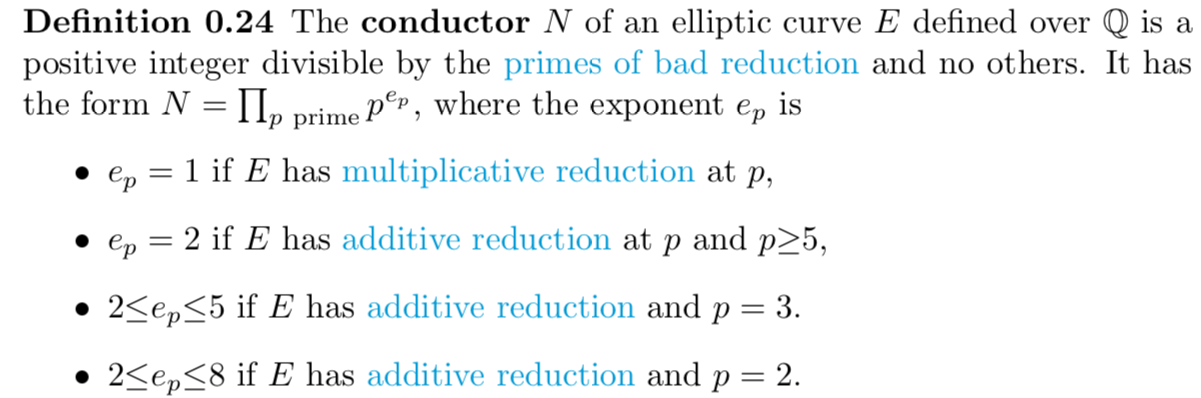
\includegraphics[width=14cm]{conductor}}
  \caption{An \sTeX Definition of the Conductor of an Elliptic
    Curve}\label{fig:conductor}
\end{figure}

\subsection{The OpenDreamKit System APIs}

We have generated and cross-linked system APIs for the computer algebra systems GAP,
SageMath, and SINGUALAR, they can be found at
\url{https://gl.mathhub.info/ODK/{GAP,SAGE,SINGULAR,LMFDB}}.\ednote{MK: write some more}

\section{Evaluation \& Conclusion}\label{sec:concl}
Figure~\ref{fig:MitM-graph} shows an overview of the MitM ontology, together with the the
system APIs and the alignments (in red) \ednote{MK: remake MitM-Graph, maybe we can add
  the SMGloM theories as well, then we could show more alignments}. We can directly see
that the MitM ontology is dwarfed the system API graphs. This is to be expected, since we
have mainly covered the background knowledge needed for the OpenDreamKit use cases. This
is in sync with the overall project plan, which mainly wants to demonstrate the
feasibility of the MitM approach to system integration, and expects the main part of the
MitM Ontology to be contributed by the mathematical community.  \ednote{MK: Write
  something about the evaluation}

\begin{figure}\centering
  \fbox{\begin{sideways}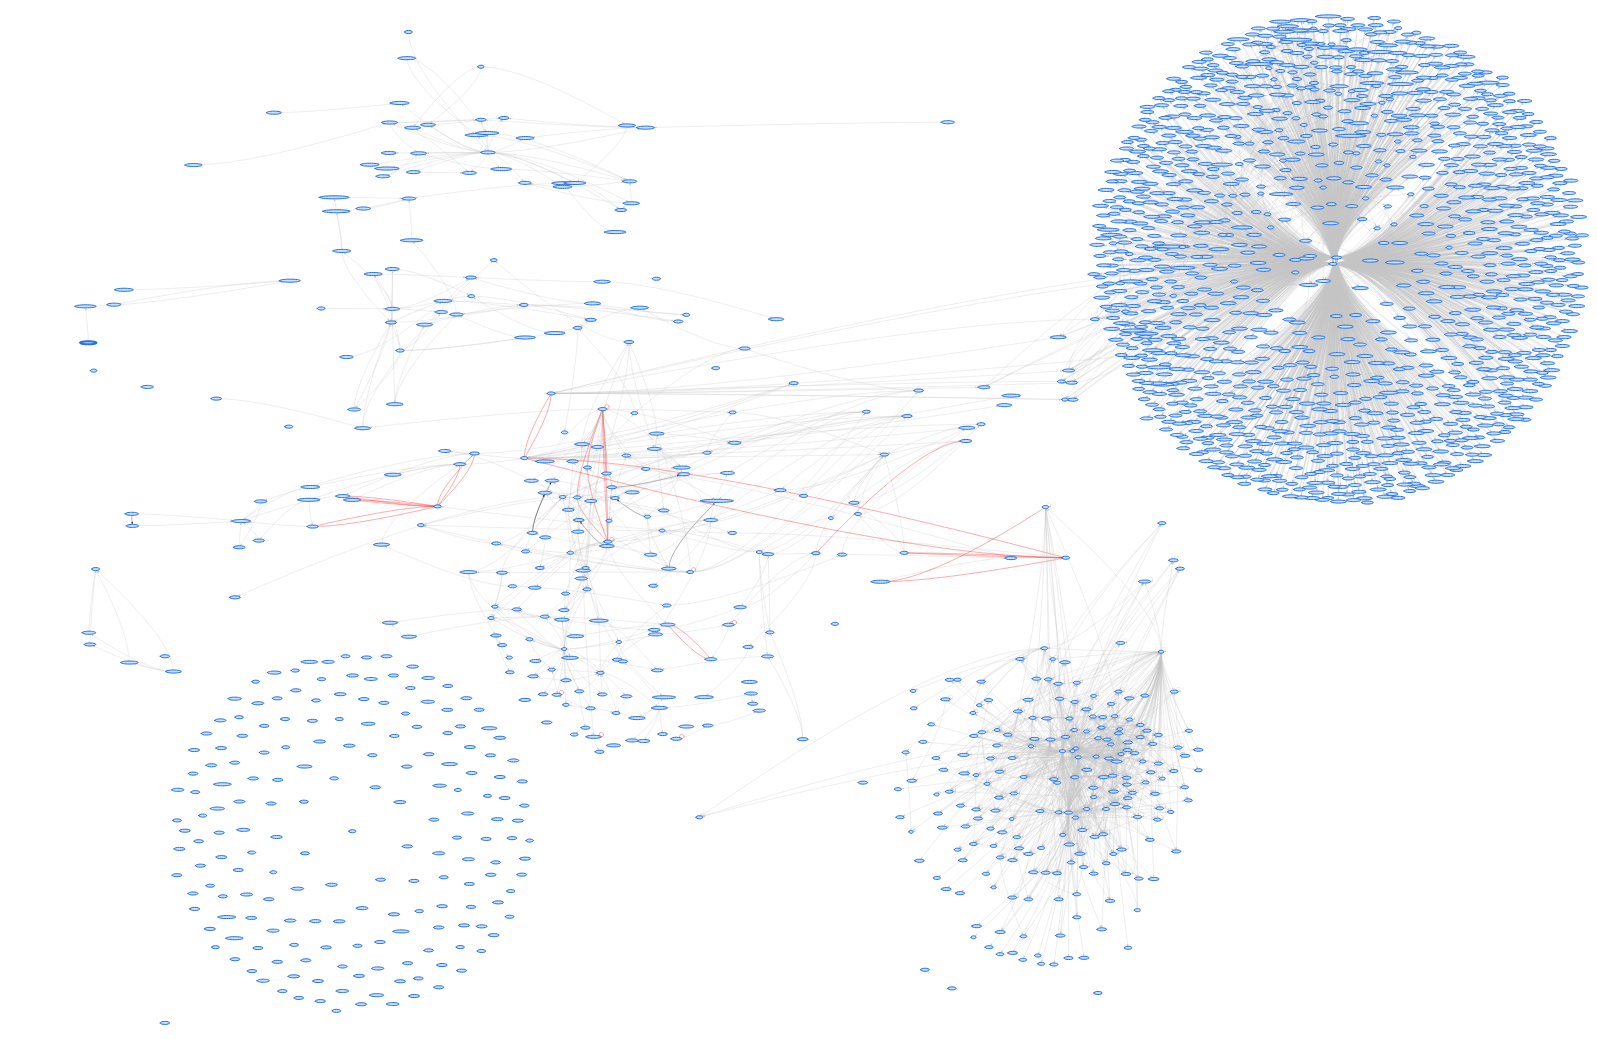
\includegraphics[width=.95\textheight]{MitM-graph}\end{sideways}}
  \caption{The MitM Theory Graph}\label{fig:MitM-graph}
\end{figure}
\printbibliography
\end{document}

%%% Local Variables:
%%% mode: latex
%%% TeX-master: t
%%% End:

%  LocalWords:  maketitle newpage tableofcontents newpage newcommand xspace ednote mathdb
%  LocalWords:  standardize dktheories concl printbibliography pn textit mmt mitm emph
%  LocalWords:  WPref dksbases prioritized taskref organized delivref dkstheories textbf
%  LocalWords:  githubissuedescription MueGauKal:cacfms17 MueRoYuRa:abtafs17 compactenum
%  LocalWords:  DehKohKon:iop16,WieKohRab:vtuimkb17,KohMuePfe:kbimss17 formalization fbox
%  LocalWords:  texttt subtyping flexary smglom stabilizes formalizations centering
%  LocalWords:  includegraphics fig:condutor textheight
